\chapter{Introduction}

\emph{"Statistics ist the explanation of variance in the light of what remains
unexplained."}

\vspace{5 mm}

Statistics was originally invented - as so many other things - by the famous mathematician C.F. Gauss, who said about his own work \emph{"Ich habe fleissig sein m\"ussen; wer es gleichfalls ist, wird eben so weit kommen"}. Even if your aspirations are not that high, you can get a lot out of statistics. In fact, if your work with real data, you probably won't be able to avoid it. Statistics can

\begin{itemize}
  \item Describe variation.
  \item Make quantitative statements about populations.
  \item Make predictions.
\end{itemize}

\textbf{Books: }There are a number of good books about statistics. My favorite is \cite{altman99}: it does not talk a lot about computers and modeling, but gives you a terrific introduction into the field. Many formulations and examples in this manuscript have been taken from that book. A more modern book, which is more voluminous and in my opinion a bit harder to read, is \cite{Riffenburgh2012}. If you are interested in a simple introduction to modern regression modeling, check out \cite{Kaplan2009}. A very good introduction to “Generalized Linear Models” is \cite{Dobson2008}. If you know your basic statistics, this is a good, advanced starter into statistical modeling.

\vspace{5 mm}

\textbf{WWW: }On the web, you find good very extensive statistics information in English under
\begin{itemize}
    \item \url{http://www.statsref.com/}
    \item \url{http://www.vassarstats.net/}
    \item \url{http://www.biostathandbook.com/}
    \item \url{http://onlinestatbook.com/2/index.html}
\end{itemize}

 A good German webpage on statistics and regulatory issues is \url{http://www.reiter1.com/}.

\vspace{5 mm}

\textbf{Exercises: }Many examples are already solved in the text. For the use in lectures (or for self-test), additional exercises are provided at the end of most chapters. For lecturers, solutions to these exercises can be provided on demand. Please contact me directly for that via email.

\section{Why Statistics?}

Statistics will help you to
\begin{itemize}
  \item Clarify the question.
  \item Identify the variable and the measure of that variable that will answer that question.
  \item Determine the required sample size.
  \item Find the correct analysis for your data.
  \item Make predictions based on your data.
\end{itemize}

Without statistics, your interpretation of your data can be massively flawed. Take for example the estimated number of German tanks during World War II, also known as the \emph{German tank problem} (\url{http://en.wikipedia.org/wiki/German_tank_problem}): from standard intelligence data, the estimate for the number of German tanks produced per month was $1550$; in contrast, the statistical estimate from the tanks observed led to a number of $327$, which was very close to the actual production number of $342$.

\chapter{Python}

\section{Getting Started}

There are three reasons why I have decided to use Python for this lecture.

\begin{enumerate}
  \item It is the most elegant programming language that I know.
  \item It is free.
  \item It is powerful.
\end{enumerate}

I have not seen many books on Python that I really liked. My favorite introductory book is \cite{Harms2010}.

There are also many tutorials available on the internet (see links below). Personally, most of the time I just google; thereby I stick primarily a) to the official pages, and b) to \url{http://stackoverflow.com/}. Also, I have found user groups surprisingly active and helpful!

\subsection{Python Links}

\begin{itemize}
  \item  \href{http://scipy-lectures.github.com}{Python Scientific Lecture Notes.} If you don't read anything else, read this!
  \item \href{http://www.scipy.org/NumPy\_for\_Matlab\_Users}{NumPy for Matlab Users} Start here if you have Matlab experience.
  \item \href{https://github.com/jrjohansson/scientific-python-lectures}{Lectures on scientific computing with Python.} Great IPython notebooks, from JR Johansson!
  \item \href{http://docs.python.org/2/tutorial}{The Python tutorial.} The official introduction.
\end{itemize}

\subsection{Free Python Books}

\begin{itemize}
  \item \href{http://swaroopch.com/notes/python}{A Byte of Python.} Free book, very good at the introductory level.
  \item \href{http://learnpythonthehardway.org/book/}{Learn Python the Hard Way, 3rd Ed} A popular, free book that you can work through.
  \item \href{http://www.greenteapress.com/thinkpython}{ThinkPython.} Free book, for advanced programmers.
  \item \href{http://www.kevinsheppard.com/images/0/09/Python_introduction.pdf}{Introduction to
      Python for Econometrics, Statistics and Data Analysis} by Kevin Sheppard: A
      good free book, which introduces Python with a focus on statistics.
\end{itemize}

\subsection{Installation and Updates}

In general, I suggest that you start out by installing a Python distribution which includes the most important libraries. Since all the Python packages required for this course are now available for Python 3.x, I will use primarily Python 3 for this book. However, all the scripts included should also work for Python 2.7. My favorite Python distributions  are

\begin{enumerate}
    \item \href{https://winpython.github.io/}{WinPython} No admin-rights required. Recommended for Windows users.
    \item \href{https://store.continuum.io/cshop/anaconda/}{anaconda} From Continuum. For Windows, Mac, and Linux.
\end{enumerate}

which are very good starting points when you are using Windows. \emph{winpython} does not require administrator rights, and \emph{anaconda} is a more recent distribution, which is free for educational purposes.

Mac and Unix users should check out the \href{https://github.com/jrjohansson/scientific-python-lectures}{installations tips from Johansson}.

\subsection{PyPI - the Python Package Index}

If you decide to install things manually, you need the following modules in addition to the Python standard library (in brackets I give the version number with which the code provided here was tested):

\begin{itemize}
  \item \emph{ipython 2.3.0} ... For interactive work.
  \item \emph{numpy 1.8.2} ... For working with vectors and arrays.
  \item \emph{scipy 0.14} ... All the essential scientific algorithms, including those for statistics.
  \item \emph{matplotlib 1.4.1} ... The de-facto standard module for plotting and visualization.
  \item \emph{pandas 0.15.0} ... Adds \emph{DataFrames} (imagine powerful spreadsheets) to Python.
  \item \emph{patsy 0.3.0} ... For working with statistical formulas.
  \item \emph{statsmodels 0.6.0} ... For statistical modeling and advanced analysis.
  \item \emph{seaborn 0.4.0} ... For visualization of statistical data.
\end{itemize}

The \href{https://pypi.python.org/pypi}{Python Package Index (\emph{PyPI})} is a repository of software for the Python programming language. There are currently 51219 packages here!

To use a package from this index you simply can use

\begin{lstlisting}
    pip install [package]
\end{lstlisting}

and to update packages

\begin{lstlisting}
    pip install [package] -U
\end{lstlisting}

To get a list of all the Python packages installed, type

\begin{lstlisting}
    pip list
\end{lstlisting}


\section{Ipython}

\begin{figure}
  \centering
  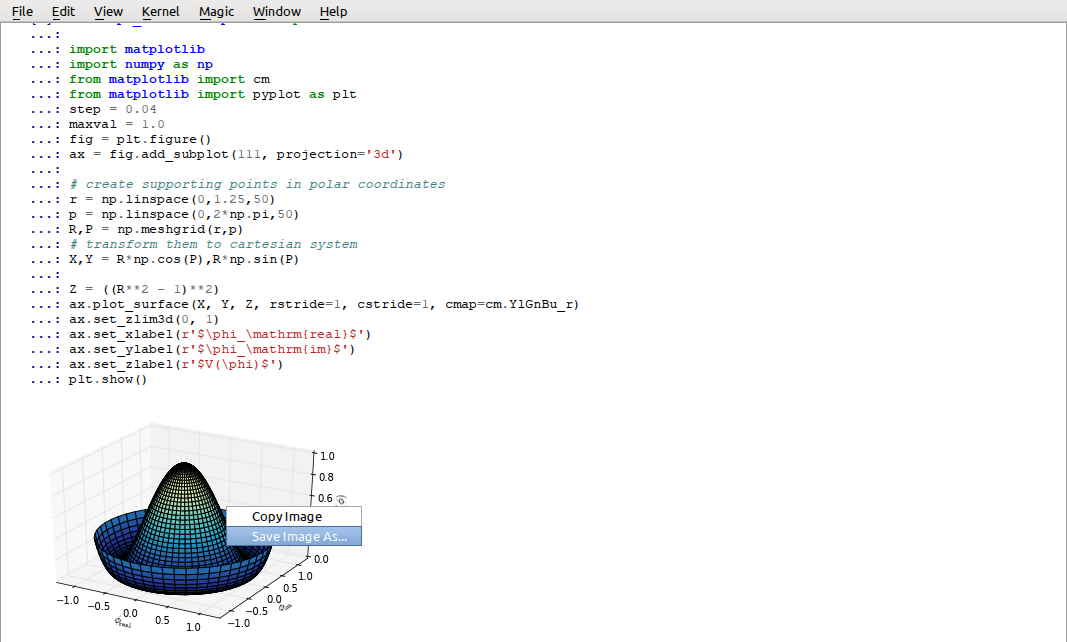
\includegraphics[width=0.75\textwidth]{../Images/ipython-qtconsole.png}\\
  \caption{The \emph{ipython qtconsole} provides a powerful and flexible interactive work environment.}
\end{figure}

Make sure that you have a good programming environment! Currently, my favorite way of programming is
similar to my old Matlab style: I first get the individual steps worked out interactively in an
\href{http://ipython.org/}{ipython} \emph{qtconsole}. Ipython \index{general}{Python!ipython} provides interactive computing with Python, similar to the commandline in Matlab. It comes with a command history, interactive data visualization, command completion, and a lot of features that make it quick and easy to try out code. When ipython is started in \emph{pylab mode} (which is the typical configuration), it automatically loads numpy and matplotlib.pyplot into the active workspace, and provides a very convenient, Matlab-like programming environment.

A very helpful new addition is the browser-based \emph{ipython notebook}, with support for code, text, mathematical expressions, inline plots and other rich media. Please check out the links to the ipython
notebooks in this statistics introduction. I believe that it will  help you to get up to speed with python much more quickly.

\subsection{Personalizing IPython}

When working on a new problem, I always start out with IPython. Once I have the individual steps working, I use the IPython command \lstinline{\%history} to get the commands I have used, and switch to an integrated development environment (typically \emph{Wing} or \emph{Spyder}).

To start up IPython quickly in the location and with the configuration I like, I use the following tricks (the following are the steps on MS Windows, but should be easy to adapt to other operating systems):

To personalize ipython, generate your own profile:

\begin{itemize}
  \item run "cmd"

  \item In the newly created command shell, execute the following command
        \begin{lstlisting}
            ipython profile create $<myName>$
        \end{lstlisting}
        (This generates a folder $.ipython \backslash profile\_<myName> \backslash startup"$)
  \item Into this folder, place a file with e.g. the name $00\_<myName>.py$, containing
        \begin{lstlisting}
        import pandas as pd
        import os
        os.chdir(r'C:\<your_favorite_dir>')"
        \end{lstlisting}
  \item Generate a file "ipython.bat" in your startup-directory, containing
      \begin{lstlisting}
      [Python-directory]\backslash Scripts \backslash ipython3 qtconsole --profile <myName> --pylab=inline
      \end{lstlisting}
\end{itemize}

Now you can start "your" ipython by just typing "ipython" in the Windows run command

To see all ipython notebooks for the course, do the following:
\begin{itemize}
  \item run "cmd"
  \item Run the commands
  \begin{lstlisting}
  cd [ipynb-directory]
  [Python-directory]\backslash Scripts \backslash ipython3.exe notebook --pylab=inline
  \end{lstlisting}
\end{itemize}



\subsection{Ipython Tips}

\begin{enumerate}
    \item Use pylab: \texttt{ipython qtconsole ---pylab=inline}
    \item For help on e.g. \texttt{plot}, use \texttt{plot?} or \texttt{help(plot)}.
    \item Check out the help tips when you start ipython.
    \item Customize ipython on your computer: it will save you time in the long run!
    \item TAB-completion, for file- and directory names, variable names, AND for commands
    \item To switch between inline and external graphs, use \texttt{\%pylab inline} and \texttt{\%pylab qt4}
    \item Use \texttt{\%runfile [aFile]} to run a file, and \texttt{import [aFile]} to import it
\end{enumerate}

\section{Developing Python Programs}

\begin{figure}
  \centering
  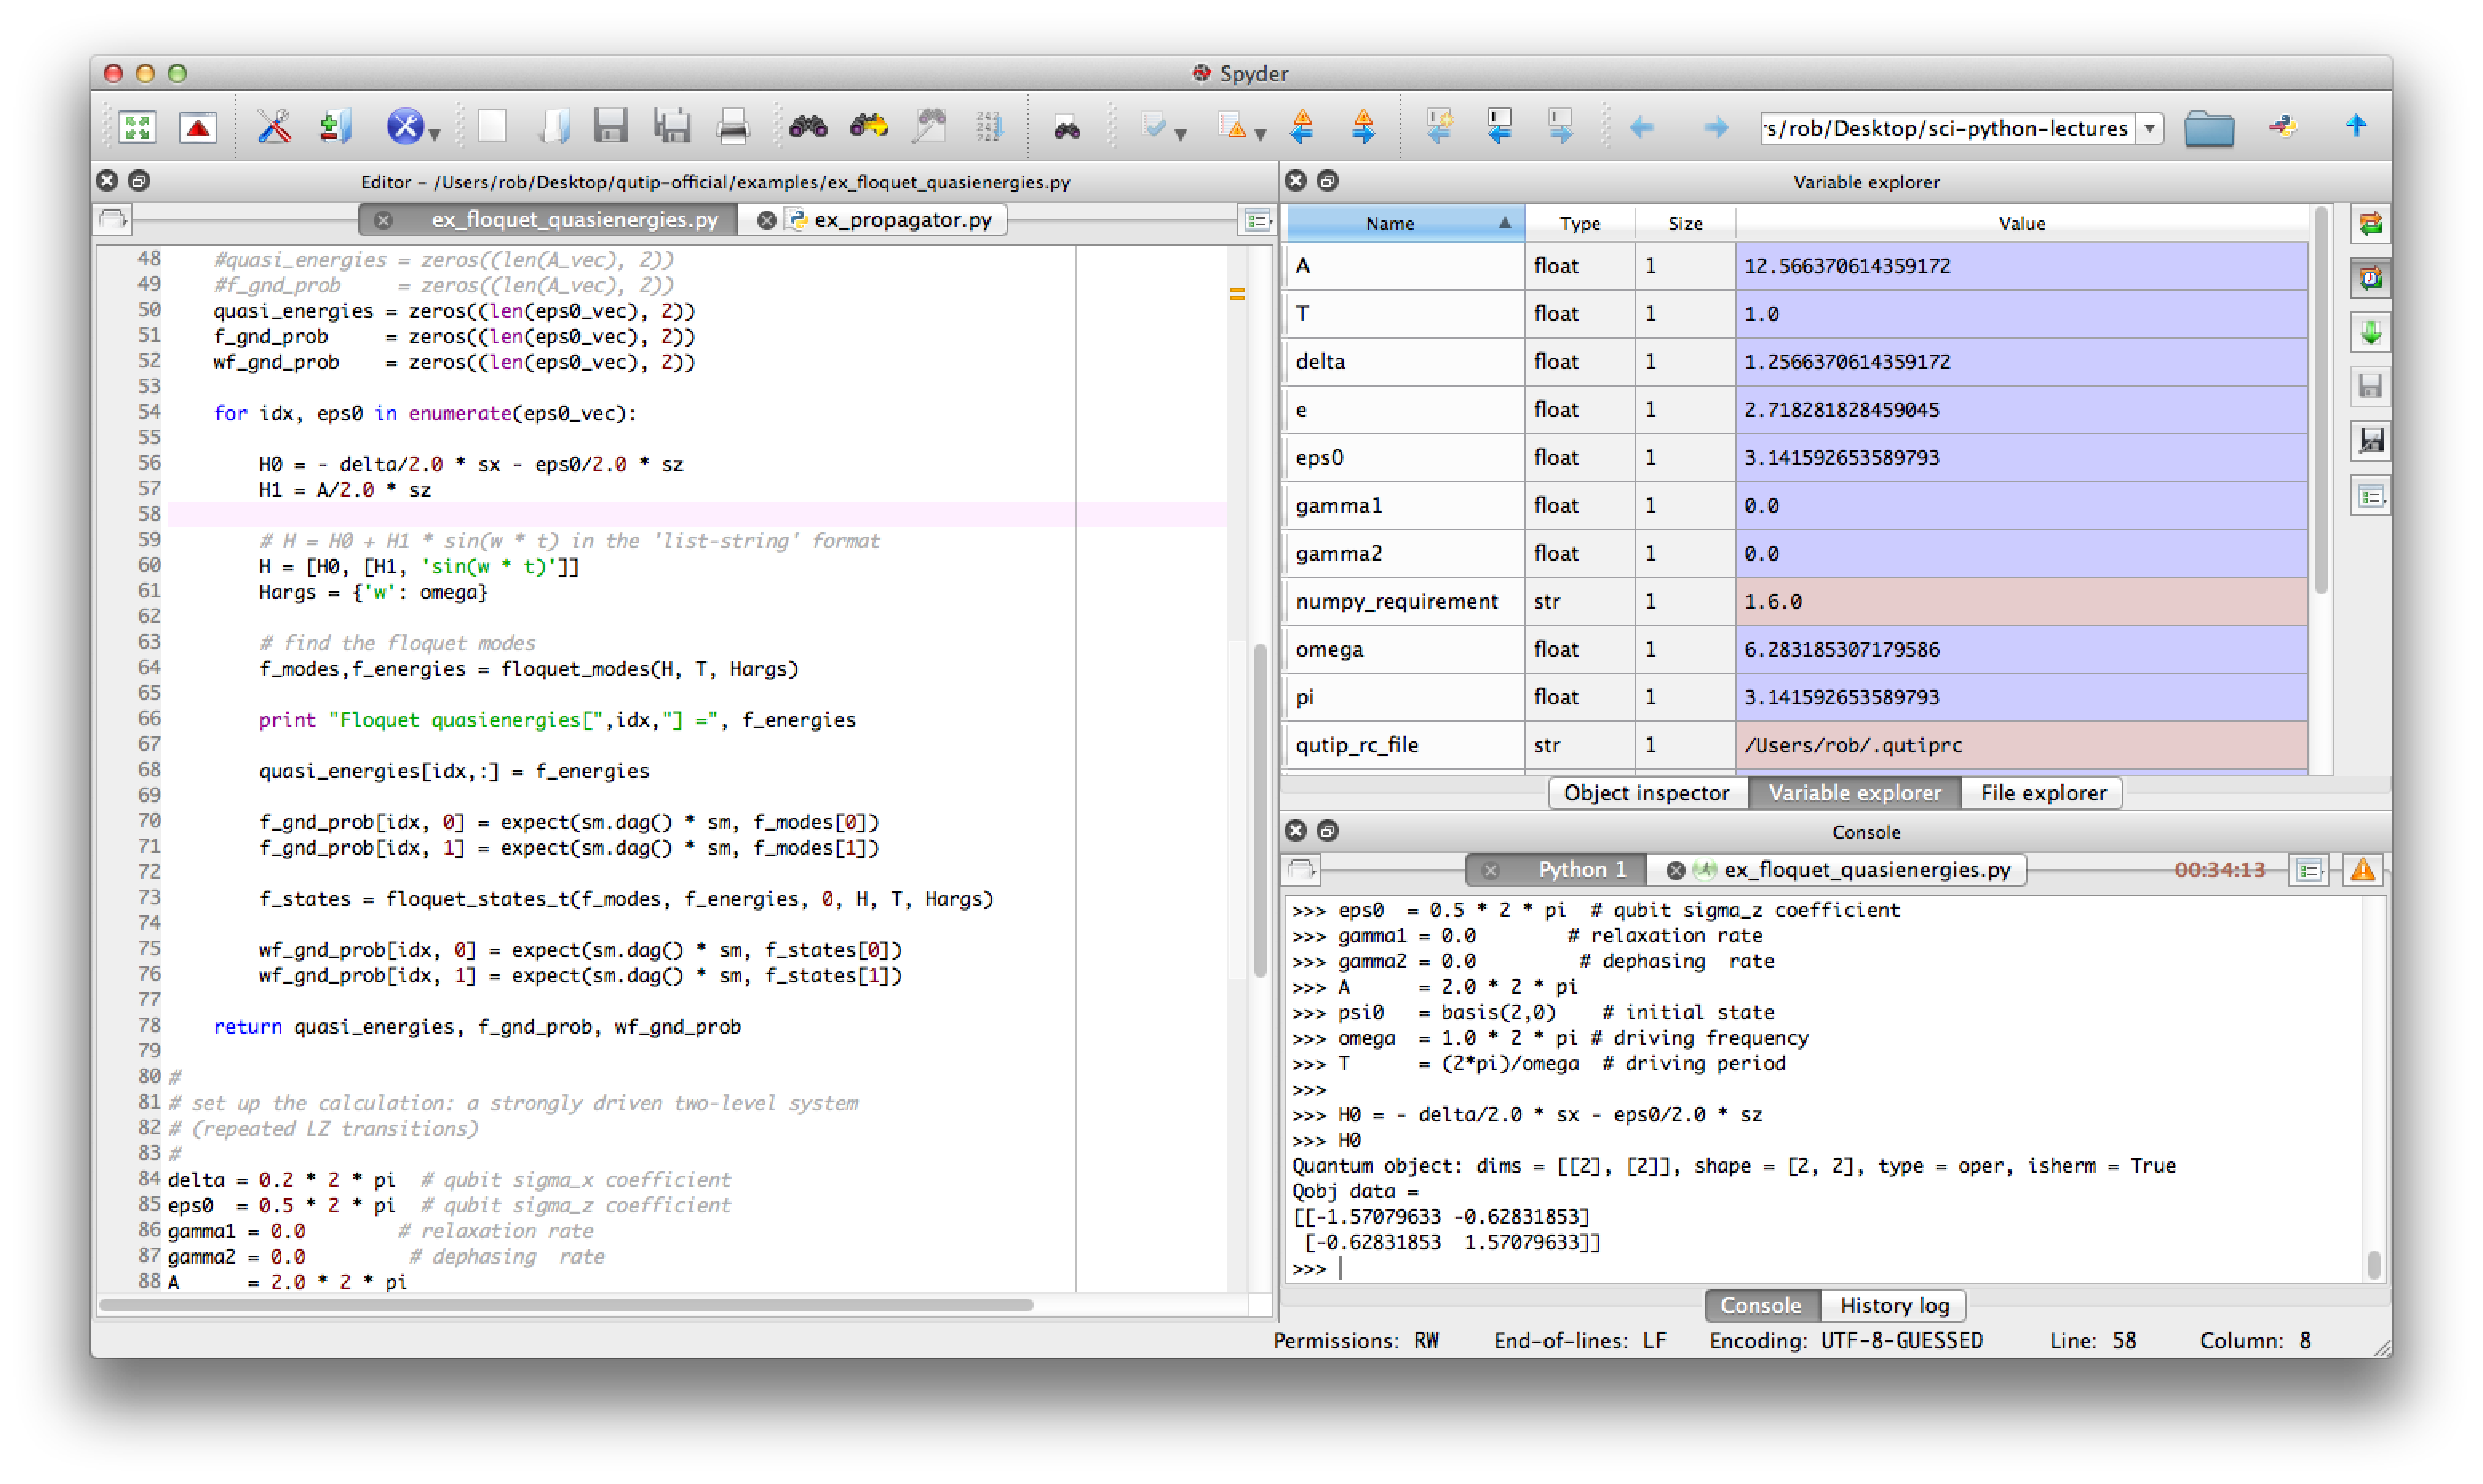
\includegraphics[width=0.75\textwidth]{../Images/spyder-screenshot.jpg}\\
  \caption{\emph{Spyder} is a very good, free IDE.}
\end{figure}

To write a program, I typically take the commands I have worked out in ipython with \lstinline{\%history}, and take them to an IDE (integrated development environment): I either use \emph{Spyder} (which is free) or \emph{Wing} (which is very good, but commercial). \emph{PyCharm} is another IDE with a good debugger, and has very good vim-emulation.

\begin{figure}
  \centering
  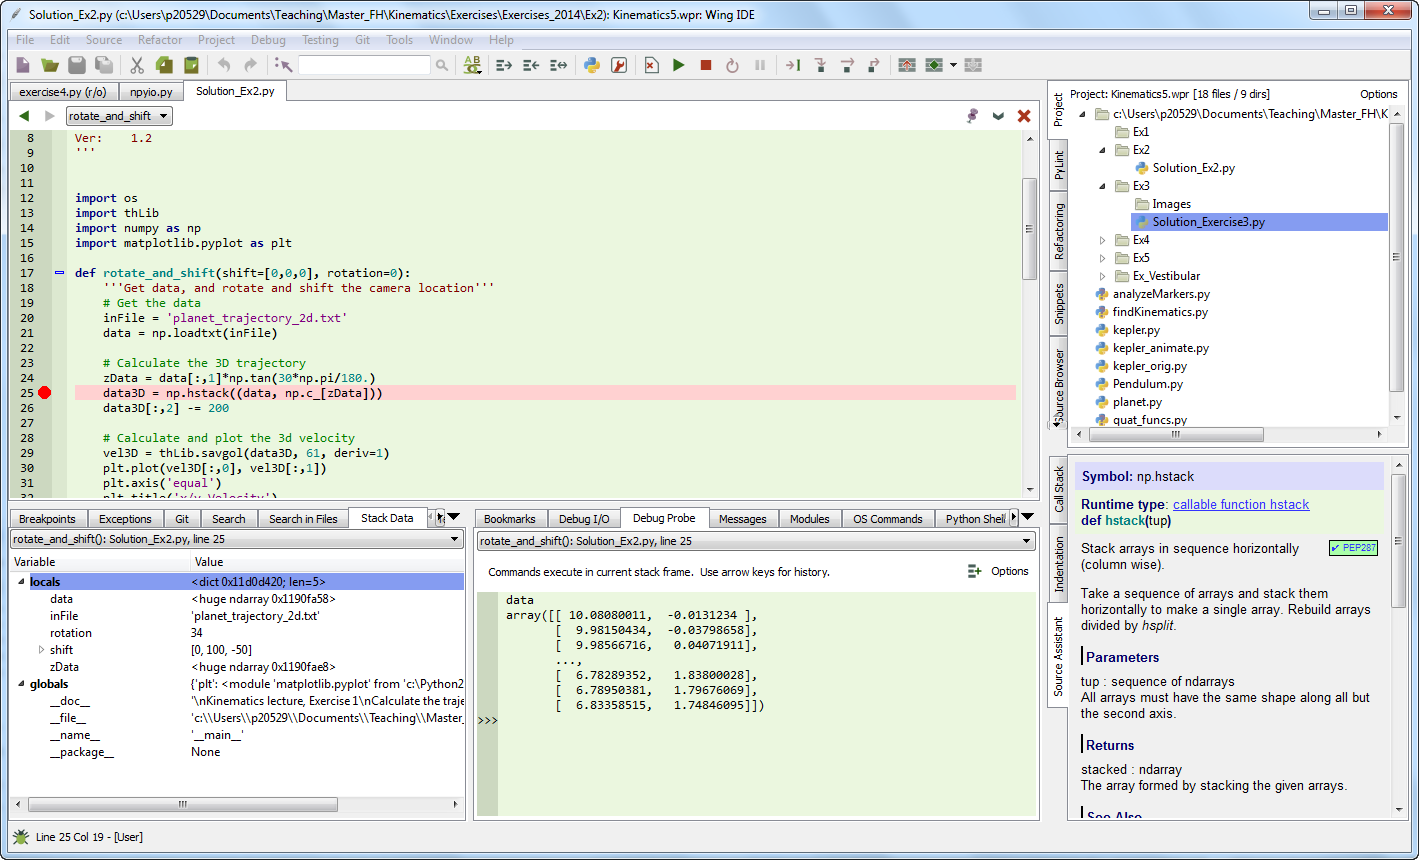
\includegraphics[width=0.75\textwidth]{../Images/Wing.png}\\
  \caption{\emph{Wing} is my favorite development environment, with probably the best existing debugger for Python.}
\end{figure}

\subsection{Python Tips}

\begin{enumerate}
  \item Stick to the standard conventions.
      \begin{itemize}
        \item Every function has a docu-string.
        \item \texttt{import matplotlib.pyplot as plt}\\
            \texttt{import numpy as np}\\
            \texttt{import scipy as sp}\\
            \texttt{import pandas as pd}\\
            \texttt{import seaborn as sns}
      \end{itemize}
  \item To get the current directory, use \texttt{os.path.abspath(os.curdir)}.
  \item Everything in Python is an object: to find out about "obj", use \texttt{type(obj)} and \texttt{dir(obj)}.
  \item Learn to use the debugger.
  \item Know \emph{lists}, \emph{tuples}, and \emph{dictionaries}; also, know about \emph{numpy arrays} and \emph{pandas DataFrames}.
  \item Use functions a lot, and understand the \texttt{if \_\_name\_\_=='\_\_main\_\_':} construct.
\end{enumerate}

\subsection{Python Data Structures}

\begin{description}
  \item[Tuple ()] A collection of different things. Cannot be modified after creation.
  \item[List [] ] A collection of similar things. Does not care if those are numbers or strings.
  \item[Array [] ] Vectors and matrices, for numerical data manipulation. Defined in \emph{numpy}.
  \item[Dictionary \{\}] Dictionaries are unordered \emph{(key/value)} collections of content, where the content is addressed as \emph{dict['key']} (see example below).
  \item[DataFrame] Data structure optimized for working with named, statistical data. Defined in \emph{pandas}. (See next chapter.)
\end{description}

\begin{lstlisting}
    In [1]: myTuple = ('abc', np.arange(0,3,0.2), 2.5)

    In [2]: myTuple[2]
    Out[2]: 2.5

    In [3]: myList = ['abc', 'def', 'ghij']

    In [4]: myList.append('klm')

    In [5]: myList2 = [1,2,3]

    In [6]: myList3 = [4,5,6]

    In [7]: myList2 + myList3
    Out[7]: [1, 2, 3, 4, 5, 6]

    In [8]: myArray = np.array(myList2)

    In [9]: myArray2 = np.array(myList3)

    In [10]: myArray + myArray2
    Out[10]: array([5, 7, 9])

    In [11]: myDict = dict(one=1, two=2, info='some information')

    In [12]: myDict2 = {'ten':1, 'twenty':20, 'info':'more information'}

    In [13]: myDict['info']
    Out[13]: 'some information'

    In [14]: myDict.keys()
    Out[14]: dict_keys(['one', 'info', 'two'])
\end{lstlisting}

\section{Matplotlib, pylab, and pyplot: how are they related?}

The flexibility of Python has the "disadvantage" that it can come in different flavors or coding styles. When you know the different approaches, they are great to use. But when you get started, it can be a bit confusing. The following section from the Matplotlib documentation may help to clarify
these things:

\textbf{Matplotlib}\index{general}{Python!Matplotlib} is the whole package; \emph{pylab} is a Matlab-like module in matplotlib that gets installed alongside matplotlib; and \emph{matplotlib.pyplot} is a module in matplotlib.

\textbf{Pyplot}\index{general}{Python!pyplot} provides the state-machine interface to the underlying plotting library in matplotlib. This means that figures and axes are implicitly and automatically created to achieve the desired plot. For example, calling \emph{plot }from pyplot will automatically create the necessary figure and axes to achieve the desired plot. Setting a \emph{title }will then automatically set that title to the current axes object:

\begin{lstlisting}
    import matplotlib.pyplot as plt

    plt.plot(np.arange(10))
    plt.title("Simple Plot")
    plt.show()
\end{lstlisting}

\textbf{Pylab}\index{general}{Python!pylab} combines the pyplot functionality (for plotting) with the numpy functionality (for mathematics and for working with arrays) in a single namespace, making that namespace (or environment) even more MATLAB-like. For example, one can call the sin and cos functions just like you could in MATLAB, as well as having all the features of pyplot.

The pyplot interface is generally preferred for non-interactive plotting (i.e., scripting). The pylab interface is convenient for interactive calculations and plotting, as it minimizes typing. Note that this is what you get if you use the ipython shell with the -pylab option, which imports everything from pylab and makes plotting fully interactive.

\section{Coding Styles in Python}

In Python you will find different coding styles and usage patterns. These styles are all perfectly valid, and each have their pros and cons. Just about all of the examples can be converted into another style and achieve the same results. The only caveat is to avoid mixing the coding styles for your own code.

Of the different styles, there are two that are officially supported. Therefore, these are the preferred ways to use matplotlib.

For the preferred pyplot style, the imports at the top of your scripts will typically be:

\begin{lstlisting}
    import matplotlib.pyplot as plt
    import numpy as np
\end{lstlisting}

Then one calls, for example, np.arange, np.zeros, np.pi, plt.figure, plt.plot, plt.show, etc. So, a simple example in this style would be:

\begin{lstlisting}
    import matplotlib.pyplot as plt
    import numpy as np
    x = np.arange(0, 10, 0.2)
    y = np.sin(x)
    plt.plot(x, y)
    plt.show()
\end{lstlisting}

Note that this example used pyplot's state-machine to automatically and implicitly create a figure and an axes. For full control of your plots and more advanced usage, use the pyplot interface for creating figures, and then use the object methods for the rest:

\begin{lstlisting}
    import matplotlib.pyplot as plt
    import numpy as np
    x = np.arange(0, 10, 0.2)
    y = np.sin(x)
    fig = plt.figure()
    ax = fig.add_subplot(111)
    ax.plot(x, y)
    plt.show()
\end{lstlisting}

Next, the same example using a pure MATLAB-style:

\begin{lstlisting}
    from pylab import *
    x = arange(0, 10, 0.2)
    y = sin(x)
    plot(x, y)
\end{lstlisting}

So, why all the extra typing as one moves away from the pure MATLAB-style? For very simple things like this example, the only advantage is academic: the wordier styles are more explicit, more clear as to where things come from and what is going on. For more complicated applications, this explicitness and clarity becomes increasingly valuable, and the richer and more complete object-oriented interface will likely make the program easier to write and maintain.

Here an example, to get you started with Python. For interactive work, it is
simplest to use the \emph{pylab mode}, as shown in the example below.

\subsection{Example-Session}

\PyImg "gettingStarted.py" (p \pageref{py:gettingStarted_ipy}) gives a short demonstration of Python for scientific data analysis.
\index{python}{gettingStarted}


\section{Pandas}

\href{http://pandas.pydata.org/.}{pandas} is a Python module which provides suitable data structures for
statistical analysis. It significantly enhances the abilities of Python for
data input, data organization, and data manipulation. In the following, I assume
that pandas has been imported with

\begin{lstlisting}
    import pandas as pd
\end{lstlisting}

A good introduction to pandas can be found under
\url{http://www.randalolson.com/2012/08/06/statistical-analysis-made-easy-in-python/}

\subsection{Data Input}

Pandas offers tools for reading and writing data between in-memory data structures and different
formats, e.g. CSV and text files, Microsoft Excel, and SQL databases. For example, if you have data
in your clipboard, you can import them directly with

\begin{lstlisting}
    data = pd.read_clipboard()
\end{lstlisting}

Or data from "Sheet1" in an Excel-file "data.xls" can be read in easily with

\begin{lstlisting}
    xls = pd.io.parsers.ExcelFile('data.xls')
    data = xls.parse('Sheet1')
\end{lstlisting}

\textbf{Example: }
\PyImg "readZip.py" (p \pageref{py:readZip}) This advanced script shows you how you can directly import data from an MS-Excel file from a zipped archive on the web.
\index{python}{readZip}

\subsection{Data Handling and Manipulation}


To handle labeled data, pandas introduces \emph{DataFrame} objects. A DataFrame is a 2-dimensional labeled data structure with columns of potentially different types. You can think of it like a spreadsheet or SQL table. It is generally the most commonly used pandas object.
At first, handling data with Pandas feels a bit unusual. To get you started, let me give you a specific example:

\begin{lstlisting}
    import numpy as np
    import pandas as pd

    t = np.arange(0,10,0.1)
    x = np.sin(t)
    y = np.cos(t)

    df = pd.DataFrame({'Time':t, 'x':x, 'y':y})
\end{lstlisting}

In Pandas, rows are addressed through "indices", and columns through their "column" name.
To address the first column only, you have two options:

\begin{lstlisting}
    df.Time
    df['Time']
\end{lstlisting}

If you want to extract two columns at the same time, you have to use a Python-list:

\begin{lstlisting}
    data = df[['Time', 'y']]
\end{lstlisting}

To display the first or last rows, use

\begin{lstlisting}
    data.head()
    data.tail()
\end{lstlisting}

For e.g. rows 5-10 (note that this are 6 numbers), use

\begin{lstlisting}
    data[4:10]
\end{lstlisting}

as $10-4=6$. (I know, the array indexing takes some time to get used to. Just keep in mind that Python addresses the \emph{locations between} entries, not the entries, and that it starts at $0$!!) To do this in one go, use

\begin{lstlisting}
    df[['Time', 'y']][4:10]
\end{lstlisting}

You can also apply the standard row/column notation, by using the method "ix":

\begin{lstlisting}
    df.ix[[0,2],4:10]
\end{lstlisting}

Finally, sometimes you want to have direct access to the data, not to the DataFrame. You can do this with

\begin{lstlisting}
    data.values
\end{lstlisting}

Pandas offers powerful functions to handle missing data and "nans", and other kinds of data manipulation like pivoting.
For example, you can use data-frames to efficiently group objects, and do a statistical evaluation of each group. The following data are simulated (but realistic) data of a survey on how many hours a day people watch on the TV, grouped into "m"ale and "f"emale responses:

\begin{lstlisting}
    data = pd.DataFrame({
        'Gender': ['f', 'f', 'm', 'f', 'm', 'm', 'f', 'm', 'f', 'm'],
        'TV': [3.4, 3.5, 2.6, 4.7, 4.1, 4.0, 5.1, 4.0, 3.7, 2.1]
        })

    # Group the data
    grouped = data.groupby('Gender')

    # Get the groups as DataFrames
    df_female = grouped.get_group('f')

    # Get the corresponding numpy-array
    values_female = grouped.get_group('f').values

    # or equivalently
    groups = grouped.groups
    values_female = groups['f']

    # Do some overview statistics
    print(grouped.describe())
\end{lstlisting}

produces

\begin{lstlisting}
                        TV
    Gender
    f      count  5.000000
           mean   4.080000
           std    0.769415
           min    3.400000
           25%    3.500000
           50%    3.700000
           75%    4.700000
           max    5.100000
    m      count  5.000000
           mean   3.360000
           std    0.939681
           min    2.100000
           25%    2.600000
           50%    4.000000
           75%    4.000000
           max    4.100000
\end{lstlisting}

For statistical analysis, pandas becomes really powerful if you combine it with \emph{statsmodels} (see below).


\section{Statsmodels}

\href{http://statsmodels.sourceforge.net/.}{statsmodels} is a Python module that provides classes and functions for the estimation of many different statistical models, as well as for conducting statistical tests, and statistical data exploration. An extensive list of result statistics are available for each estimator. \emph{statsmodels} also allows the formulation of models with the popular formula language also used by $R$, the leading statistics package. For example, data on the connection between academic "success", "intelligence" and "diligence" can be described with the model

\begin{equation*}
    success \sim intelligence * diligence
\end{equation*}

 which would capture the direct effect of "intelligence" and "diligence", as well as the interaction. You find more information on that topic in the section "Statistical Models".

While for complex statistical models R still has an edge, python has a much clearer and more readable syntax, and is arguably more powerful for the data manipulation often required for statistical analysis.

\PyImg "statsmodelsIntro.py" (p \pageref{py:statsmodelsIntro}) shows you how the combination of pandas and statsmodels can be used for data analysis.
\index{python}{statsmodelsIntro}

\section{Seaborn}

\href{http://statsmodels.sourceforge.net/.}{seaborn} is a Python visualization library based on matplotlib. Its primary goal is to provide a concise, high-level interface for drawing statistical graphics that are both informative and attractive.

\begin{lstlisting}
        x = linspace(1, 7, 50)
        y = 3 + 2*x + 1.5*randn(len(x))
        sns.regplot(x,y)
\end{lstlisting}

already produces a nice and informative regression plot

\begin{figure}[ht]
  \centering
  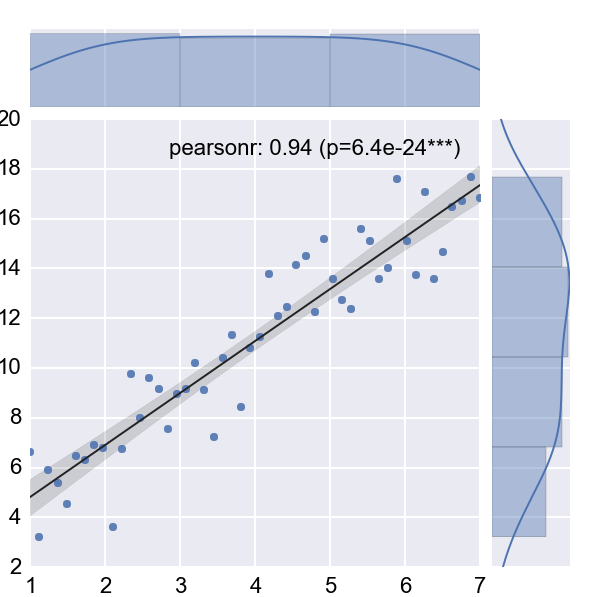
\includegraphics[width=0.5\textwidth]{../Images/regplot.png}\\
  \caption{Regression plot, from \emph{seaborn}, with a substantial amount of added information.}
\end{figure}

\subsection{General Routines}
Here is also a good place to introduce the short function that we will use a number of times to simplify the reading in of data:

\PyImg "getData.py" (p \pageref{py:getData}) Gets the input data for many Python programs in this script.
\index{python}{getData}

\section{Exercises}

\begin{itemize}
  \item Read in data from different sources:
  \begin{itemize}
    \item A CVS-file with a header ('Data\textbackslash Swimming\textbackslash swimming\_100m.csv')
    \item An MS-Excel file ('Data\textbackslash data\_dobson\textbackslash GLM\_data\textbackslash Table 2.8 Waist loss.xls')
    \item Data from the WWW (see "readZip.py" \ref{py:readZip})
  \end{itemize}
  \item
  \begin{itemize}
      \item Generate a pandas dataframe, with the x-column time stamps from 0 to 10 sec, at a rate of 10 Hz, the y-column data values with a sine with 1.5 Hz, and the z-column the corresponding cosine values. Label the x-column "Xvals", and the y-column "YVals", and the z-column "ZVals".
      \item Show the head of this dataframe
      \item Extract the data in lines 10-15 from "Yvals" and "ZVals", and write them to the file "out.txt".
  \end{itemize}
\end{itemize}
